%!TeX root=../wowtop.tex

\ArtChapter[In the Storm]{10head}

\lettrine[lines=4,findent=2pt]{L}{eatherhead} is about twelve miles from Maybury Hill. The scent of hay was in the air through the lush meadows beyond Pyrford, and the hedges on either side were sweet and gay with multitudes of dog-roses. The heavy firing that had broken out while we were driving down Maybury Hill ceased as abruptly as it began, leaving the evening very peaceful and still. We got to Leatherhead without misadventure about nine o'clock, and the horse had an hour's rest while I took supper with my cousins and commended my wife to their care.

My wife was curiously silent throughout the drive, and seemed oppressed with forebodings of evil. I talked to her reassuringly, pointing out that the Martians were tied to the pit by sheer heaviness, and at the utmost could but crawl a little out of it; but she answered only in monosyllables. Had it not been for my promise to the innkeeper, she would, I think, have urged me to stay in Leatherhead that night. Would that I had! Her face, I remember, was very white as we parted.

For my own part, I had been feverishly excited all day. Something very like the war fever that occasionally runs through a civilised community had got into my blood, and in my heart I was not so very sorry that I had to return to Maybury that night. I was even afraid that that last fusillade I had heard might mean the extermination of our invaders from Mars. I can best express my state of mind by saying that I wanted to be in at the death.

It was nearly eleven when I started to return. The night was unexpectedly dark; to me, walking out of the lighted passage of my cousins' house, it seemed indeed black, and it was as hot and close as the day. Overhead the clouds were driving fast, albeit not a breath stirred the shrubs about us. My cousins' man lit both lamps. Happily, I knew the road intimately. My wife stood in the light of the doorway, and watched me until I jumped up into the dog cart. Then abruptly she turned and went in, leaving my cousins side by side wishing me good hap.

I was a little depressed at first with the contagion of my wife's fears, but very soon my thoughts reverted to the Martians. At that time I was absolutely in the dark as to the course of the evening's fighting. I did not know even the circumstances that had precipitated the conflict. As I came through Ockham (for that was the way I returned, and not through Send and Old Woking) I saw along the western horizon a blood-red glow, which as I drew nearer, crept slowly up the sky. The driving clouds of the gathering thunderstorm mingled there with masses of black and red smoke.

Ripley Street was deserted, and except for a lighted window or so the village showed not a sign of life; but I narrowly escaped an accident at the corner of the road to Pyrford, where a knot of people stood with their backs to me. They said nothing to me as I passed. I do not know what they knew of the things happening beyond the hill, nor do I know if the silent houses I passed on my way were sleeping securely, or deserted and empty, or harassed and watching against the terror of the night.

From Ripley until I came through Pyrford I was in the valley of the Wey, and the red glare was hidden from me. As I ascended the little hill beyond Pyrford Church\label{cylinder3a} the glare came into view again, and the trees about me shivered with the first intimation of the storm that was upon me. Then I heard midnight pealing out from Pyrford Church behind me, and then came the silhouette of Maybury Hill, with its tree-tops and roofs black and sharp against the red.

Even as I beheld this a lurid green glare lit the road about me and showed the distant woods towards Addlestone.\label{cylinder3b} I felt a tug at the reins. I saw that the driving clouds had been pierced as it were by a thread of green fire, suddenly lighting their confusion and falling into the field to my left. It was the third falling star!

Close on its apparition, and blindingly violet by contrast, danced out the first lightning of the gathering storm, and the thunder burst like a rocket overhead. The horse took the bit between his teeth and bolted.

A moderate incline runs towards the foot of Maybury Hill, and down this we clattered. Once the lightning had begun, it went on in as rapid a succession of flashes as I have ever seen. The thunderclaps, treading one on the heels of another and with a strange crackling accompaniment, sounded more like the working of a gigantic electric machine than the usual detonating reverberations. The flickering light was blinding and confusing, and a thin hail smote gustily at my face as I drove down the slope.

At first I regarded little but the road before me, and then abruptly my attention was arrested by something that was moving rapidly down the opposite slope of Maybury Hill. At first I took it for the wet roof of a house, but one flash following another showed it to be in swift rolling movement. It was an elusive vision—a moment of bewildering darkness, and then, in a flash like daylight, the red masses of the Orphanage near the crest of the hill, the green tops of the pine trees, and this problematical object came out clear and sharp and bright.

And this Thing I saw! How can I describe it? A monstrous tripod, higher than many houses, striding over the young pine trees, and smashing them aside in its career; a walking engine of glittering metal, striding now across the heather; articulate ropes of steel dangling from it, and the clattering tumult of its passage mingling with the riot of the thunder. A flash, and it came out vividly, heeling over one way with two feet in the air, to vanish and reappear almost instantly as it seemed, with the next flash, a hundred yards nearer. Can you imagine a milking stool tilted and bowled violently along the ground? That was the impression those instant flashes gave. But instead of a milking stool imagine it a great body of machinery on a tripod stand.

Then suddenly the trees in the pine wood ahead of me were parted, as brittle reeds are parted by a man thrusting through them; they were snapped off and driven headlong, and a second huge tripod appeared, rushing, as it seemed, headlong towards me. And I was galloping hard to meet it! At the sight of the second monster my nerve went altogether. Not stopping to look again, I wrenched the horse's head hard round to the right and in another moment the dog cart had heeled over upon the horse; the shafts smashed noisily, and I was flung sideways and fell heavily into a shallow pool of water.

I crawled out almost immediately, and crouched, my feet still in the water, under a clump of furze. The horse lay motionless (his neck was broken, poor brute!) and by the lightning flashes I saw the black bulk of the overturned dog cart and the silhouette of the wheel still spinning slowly. In another moment the colossal mechanism went striding by me, and passed uphill towards Pyrford.

Seen nearer, the Thing was incredibly strange, for it was no mere insensate machine driving on its way. Machine it was, with a ringing metallic pace, and long, flexible, glittering tentacles (one of which gripped a young pine tree) swinging and rattling about its strange body. It picked its road as it went striding along, and the brazen hood that surmounted it moved to and fro with the inevitable suggestion of a head looking about. Behind the main body was a huge mass of white metal like a gigantic fisherman's basket, and puffs of green smoke squirted out from the joints of the limbs as the monster swept by me. And in an instant it was gone.

So much I saw then, all vaguely for the flickering of the lightning, in blinding highlights and dense black shadows.

As it passed it set up an exultant deafening howl that drowned the thunder—»Aloo! Aloo!«—and in another minute it was with its companion, half a mile away, stooping over something in the field. I have no doubt this Thing in the field was the third of the ten cylinders they had fired at us from Mars.

\begin{wrapfigure}{O}{0.5\textwidth}
\centering
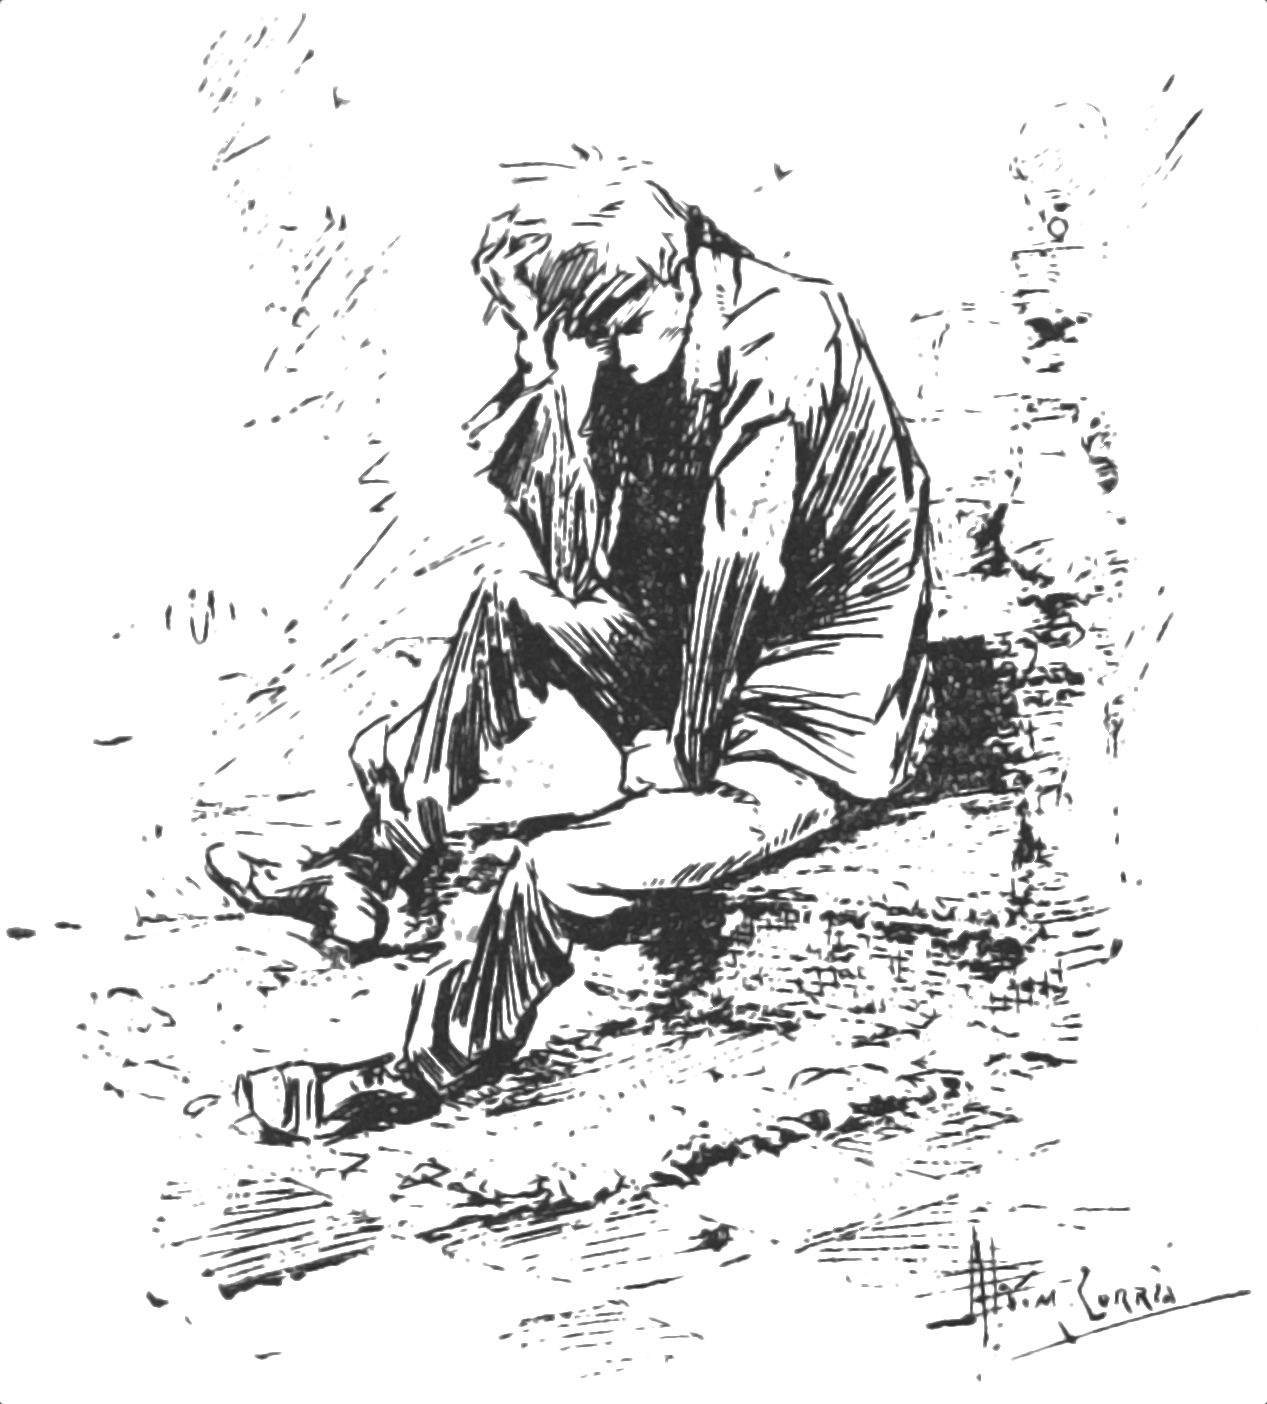
\includegraphics[width=0.5\textwidth]{10tailpiece}
\end{wrapfigure}

For some minutes I lay there in the rain and darkness watching, by the intermittent light, these monstrous beings of metal moving about in the distance over the hedge tops. A thin hail was now beginning, and as it came and went their figures grew misty and then flashed into clearness again. Now and then came a gap in the lightning, and the night swallowed them up.

I was soaked with hail above and puddle water below. It was some time before my blank astonishment would let me struggle up the bank to a drier position, or think at all of my imminent peril.

Not far from me was a little one-roomed squatter's hut of wood, surrounded by a patch of potato garden. I struggled to my feet at last, and, crouching and making use of every chance of cover, I made a run for this. I hammered at the door, but I could not make the people hear (if there were any people inside), and after a time I desisted, and, availing myself of a ditch for the greater part of the way, succeeded in crawling, unobserved by these monstrous machines, into the pine woods towards Maybury.

Under cover of this I pushed on, wet and shivering now, towards my own house. I walked among the trees trying to find the footpath. It was very dark indeed in the wood, for the lightning was now becoming infrequent, and the hail, which was pouring down in a torrent, fell in columns through the gaps in the heavy foliage.

If I had fully realised the meaning of all the things I had seen I should have immediately worked my way round through Byfleet to Street Cobham, and so gone back to rejoin my wife at Leatherhead. But that night the strangeness of things about me, and my physical wretchedness, prevented me, for I was bruised, weary, wet to the skin, deafened and blinded by the storm.

% \begin{sidewaysfigure}
% 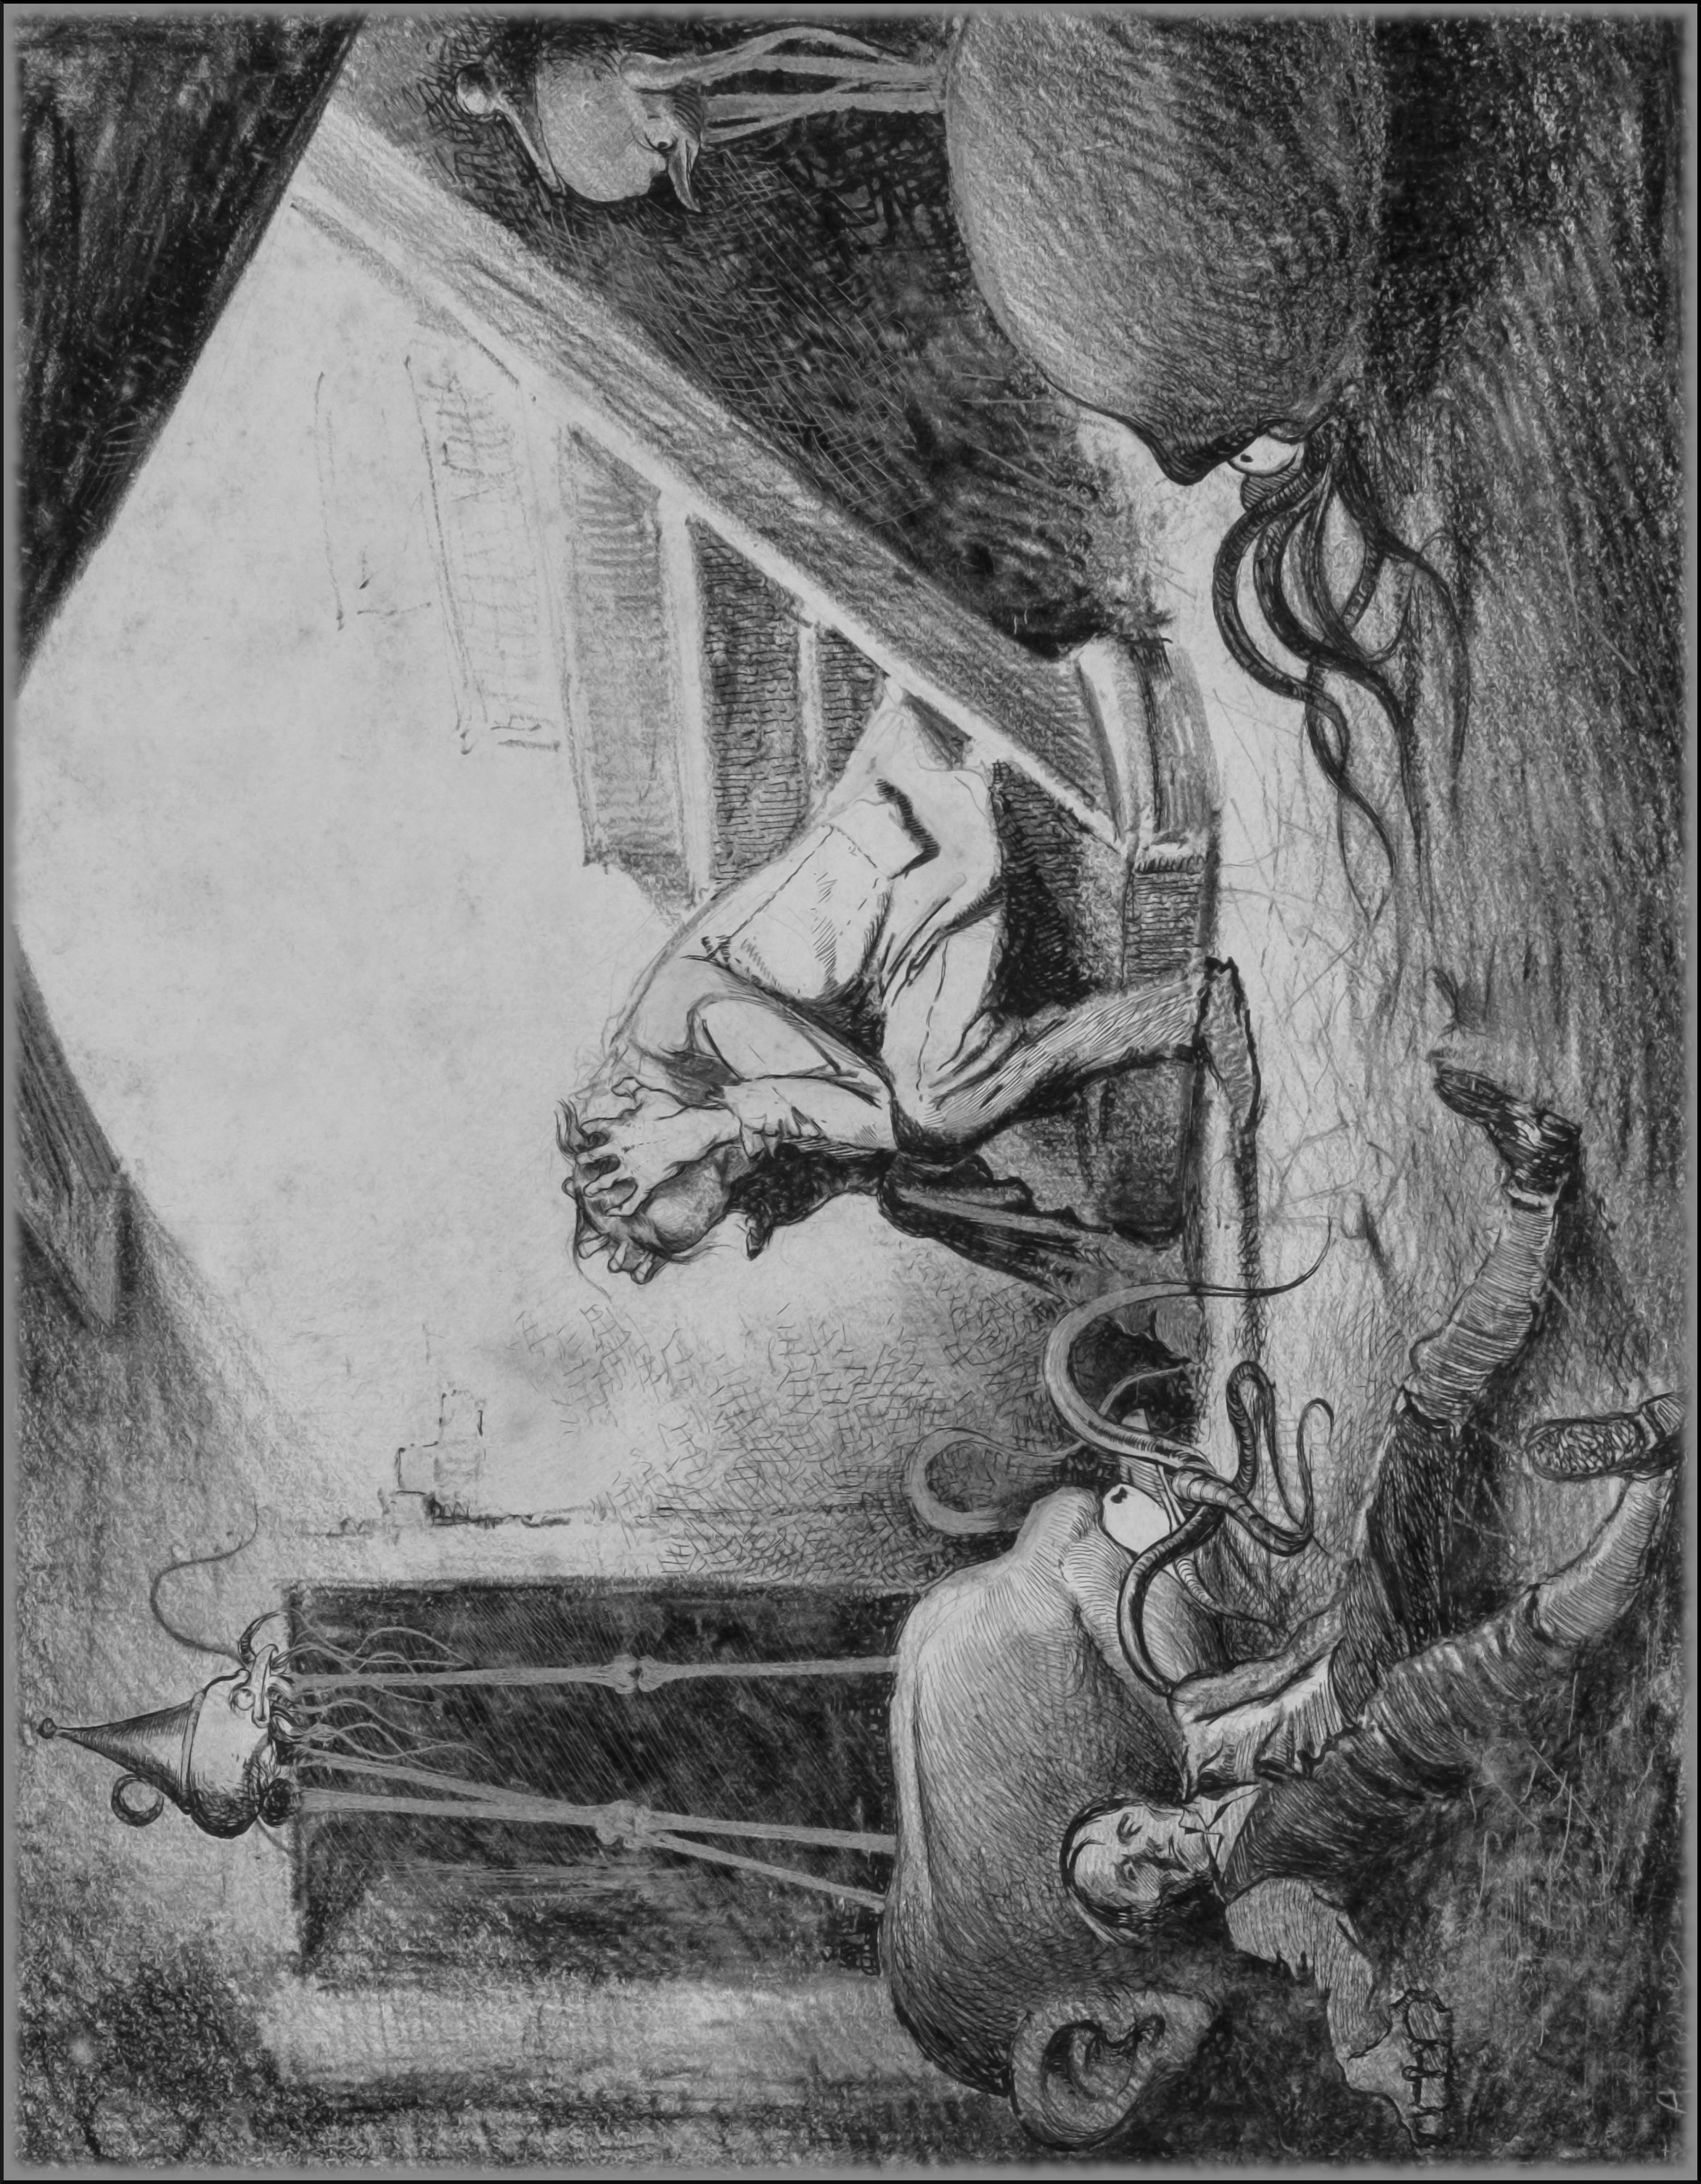
\includegraphics[width=.8\columnwidth]{10imagination}
% \caption{My imagination was full of those striding metallic monsters}
% \end{sidewaysfigure}


%\begin{figure}[tbh]
%\centering
%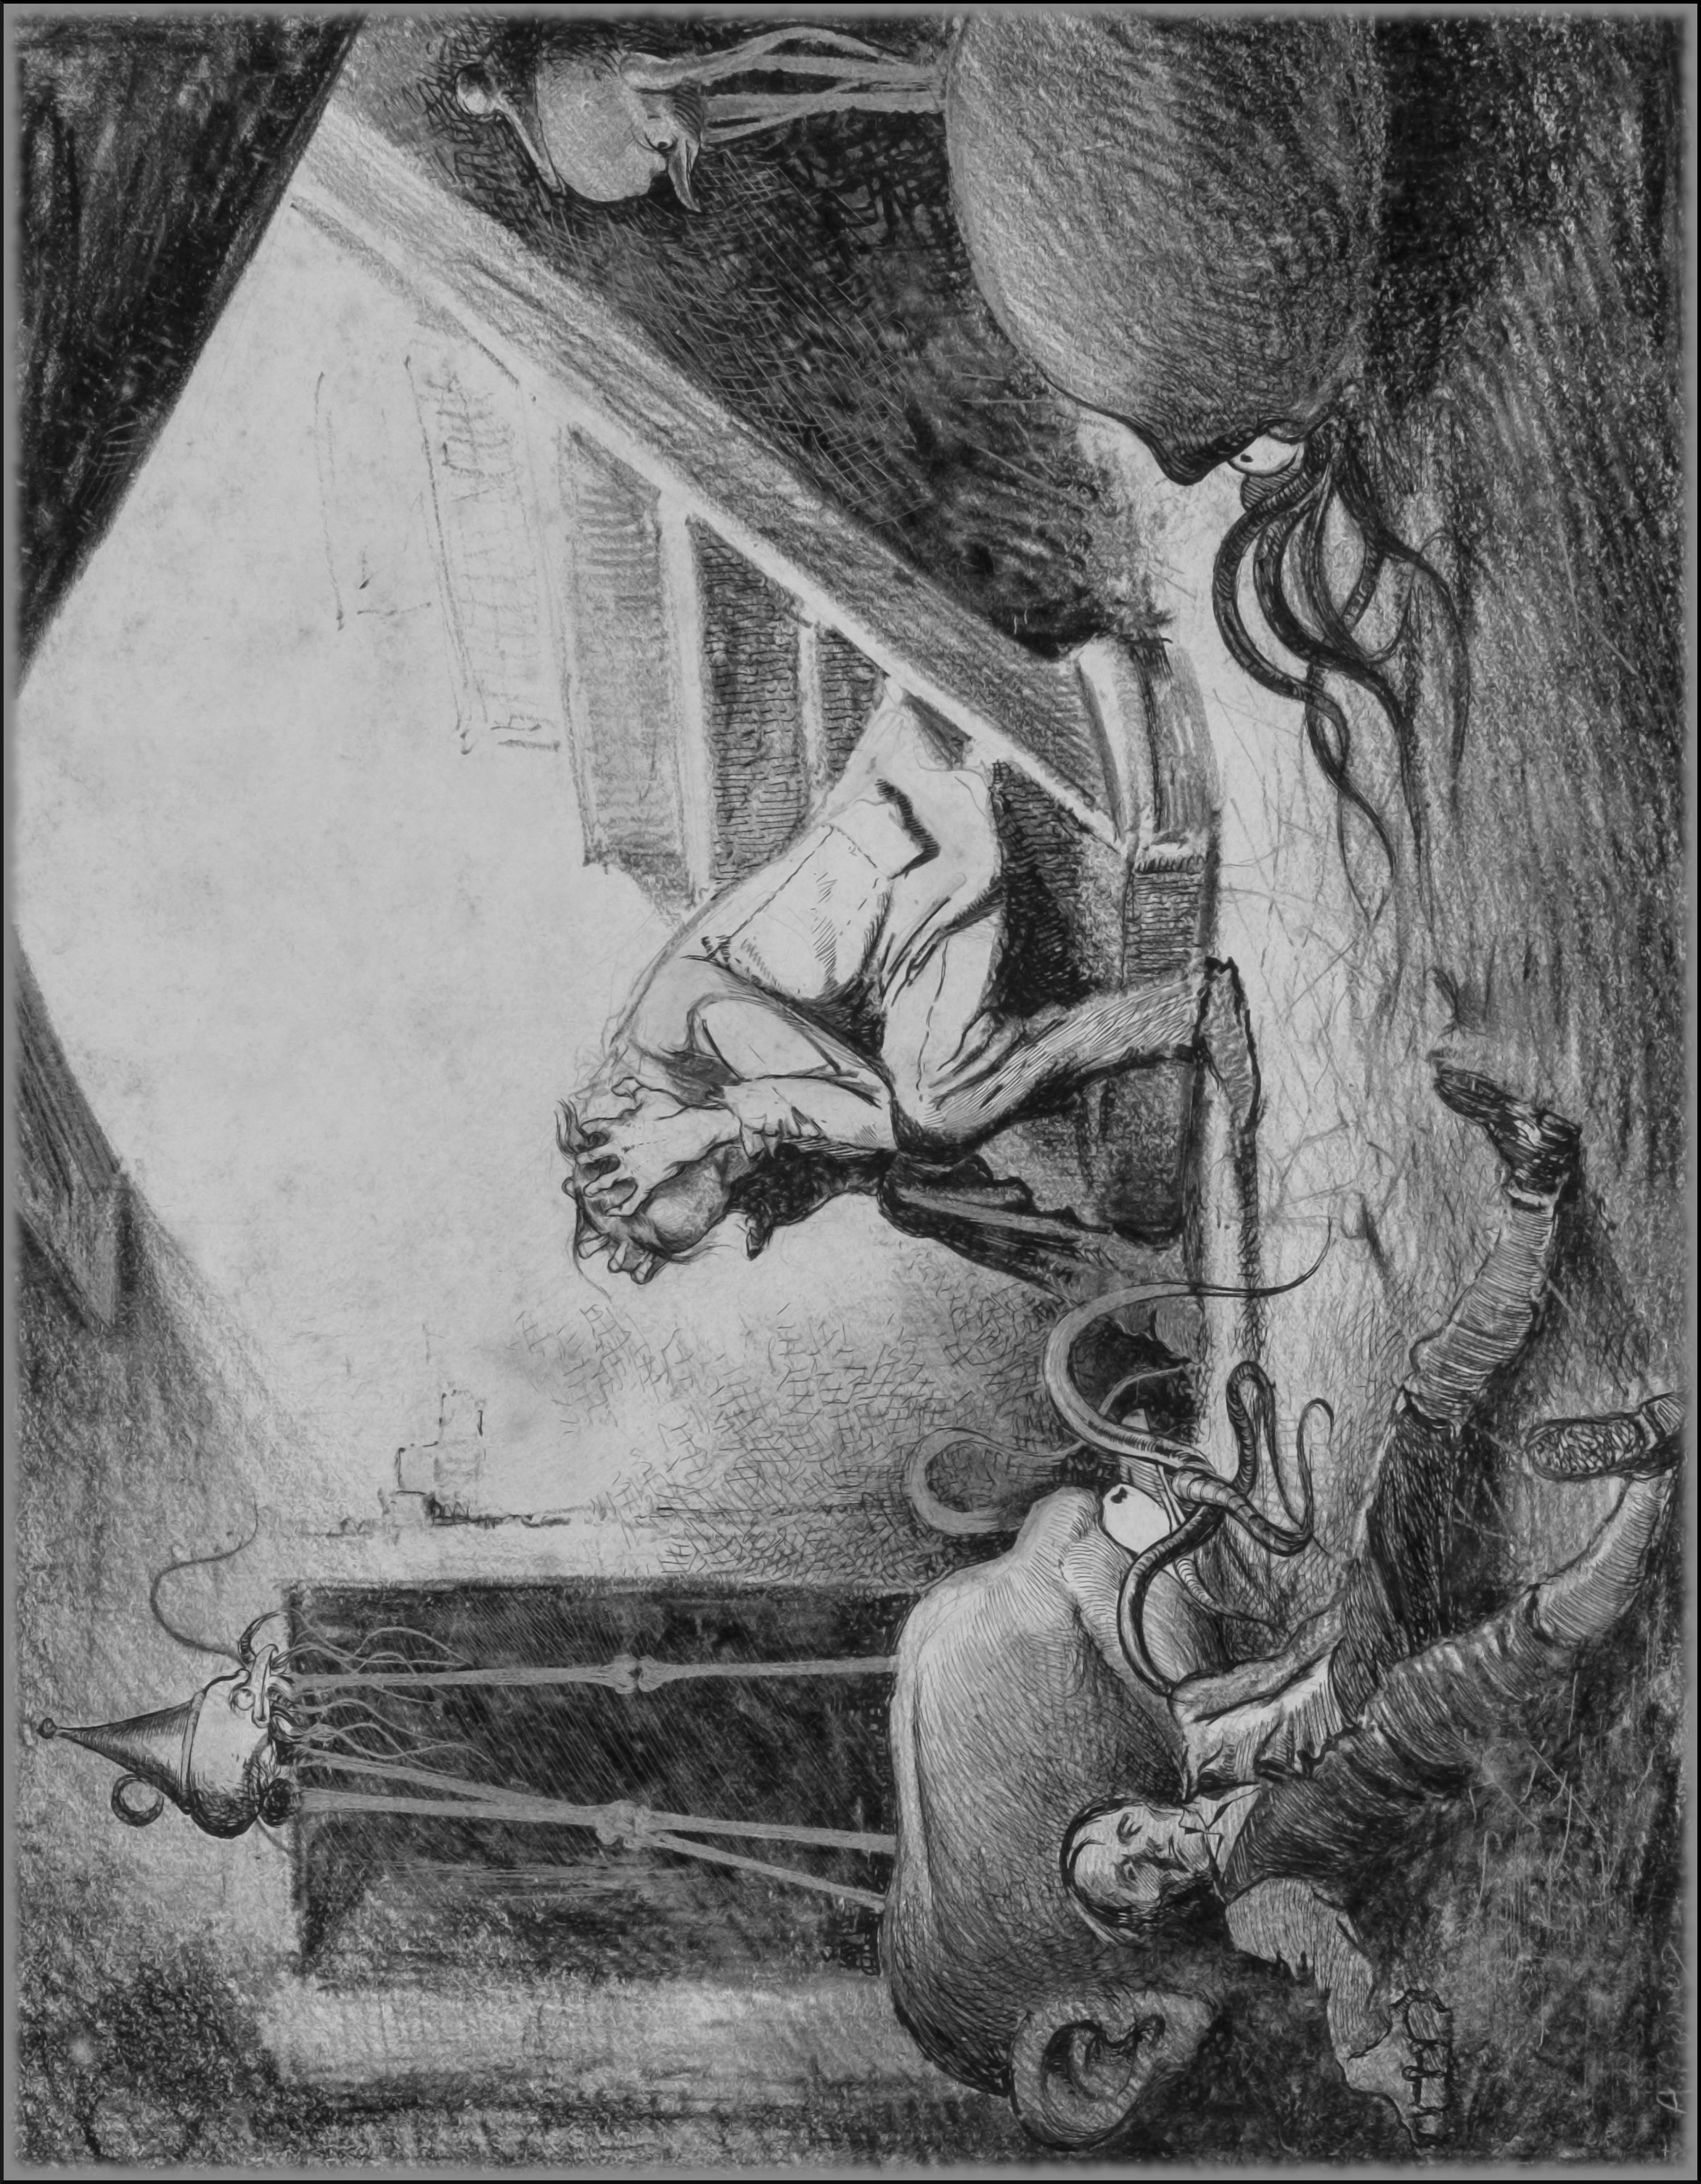
\includegraphics[width=\linewidth]{10imagination}
%\caption{My imagination was full of those striding metallic monsters}
%\end{figure}


I had a vague idea of going on to my own house, and that was as much motive as I had. I staggered through the trees, fell into a ditch and bruised my knees against a plank, and finally splashed out into the lane that ran down from the College Arms. I say splashed, for the storm water was sweeping the sand down the hill in a muddy torrent. There in the darkness a man blundered into me and sent me reeling back.

He gave a cry of terror, sprang sideways, and rushed on before I could gather my wits sufficiently to speak to him. So heavy was the stress of the storm just at this place that I had the hardest task to win my way up the hill. I went close up to the fence on the left and worked my way along its palings.

Near the top I stumbled upon something soft, and, by a flash of lightning, saw between my feet a heap of black broadcloth and a pair of boots. Before I could distinguish clearly how the man lay, the flicker of light had passed. I stood over him waiting for the next flash. When it came, I saw that he was a sturdy man, cheaply but not shabbily dressed; his head was bent under his body, and he lay crumpled up close to the fence, as though he had been flung violently against it.

Overcoming the repugnance natural to one who had never before touched a dead body, I stooped and turned him over to feel for his heart. He was quite dead. Apparently his neck had been broken. The lightning flashed for a third time, and his face leaped upon me. I sprang to my feet. It was the landlord of the »Spotted Dog«, whose conveyance I had taken.

I stepped over him gingerly and pushed on up the hill. I made my way by the police station and the College Arms towards my own house. Nothing was burning on the hillside, though from the common there still came a red glare and a rolling tumult of ruddy smoke beating up against the drenching hail. So far as I could see by the flashes, the houses about me were mostly uninjured. By the College Arms a dark heap lay in the road.

Down the road towards Maybury Bridge there were voices and the sound of feet, but I had not the courage to shout or to go to them. I let myself in with my latchkey, closed, locked and bolted the door, staggered to the foot of the staircase, and sat down. My imagination was full of those striding metallic monsters, and of the dead body smashed against the fence.


I crouched at the foot of the staircase with my back to the wall, shivering violently.
%\clearpage



\begin{pictures} 
	\begin{letter}
		\clearpage
		\begin{tikzpicture}[remember picture, overlay]
			\node (img) at ($(current page.center)+(-0.5cm,0cm)$) {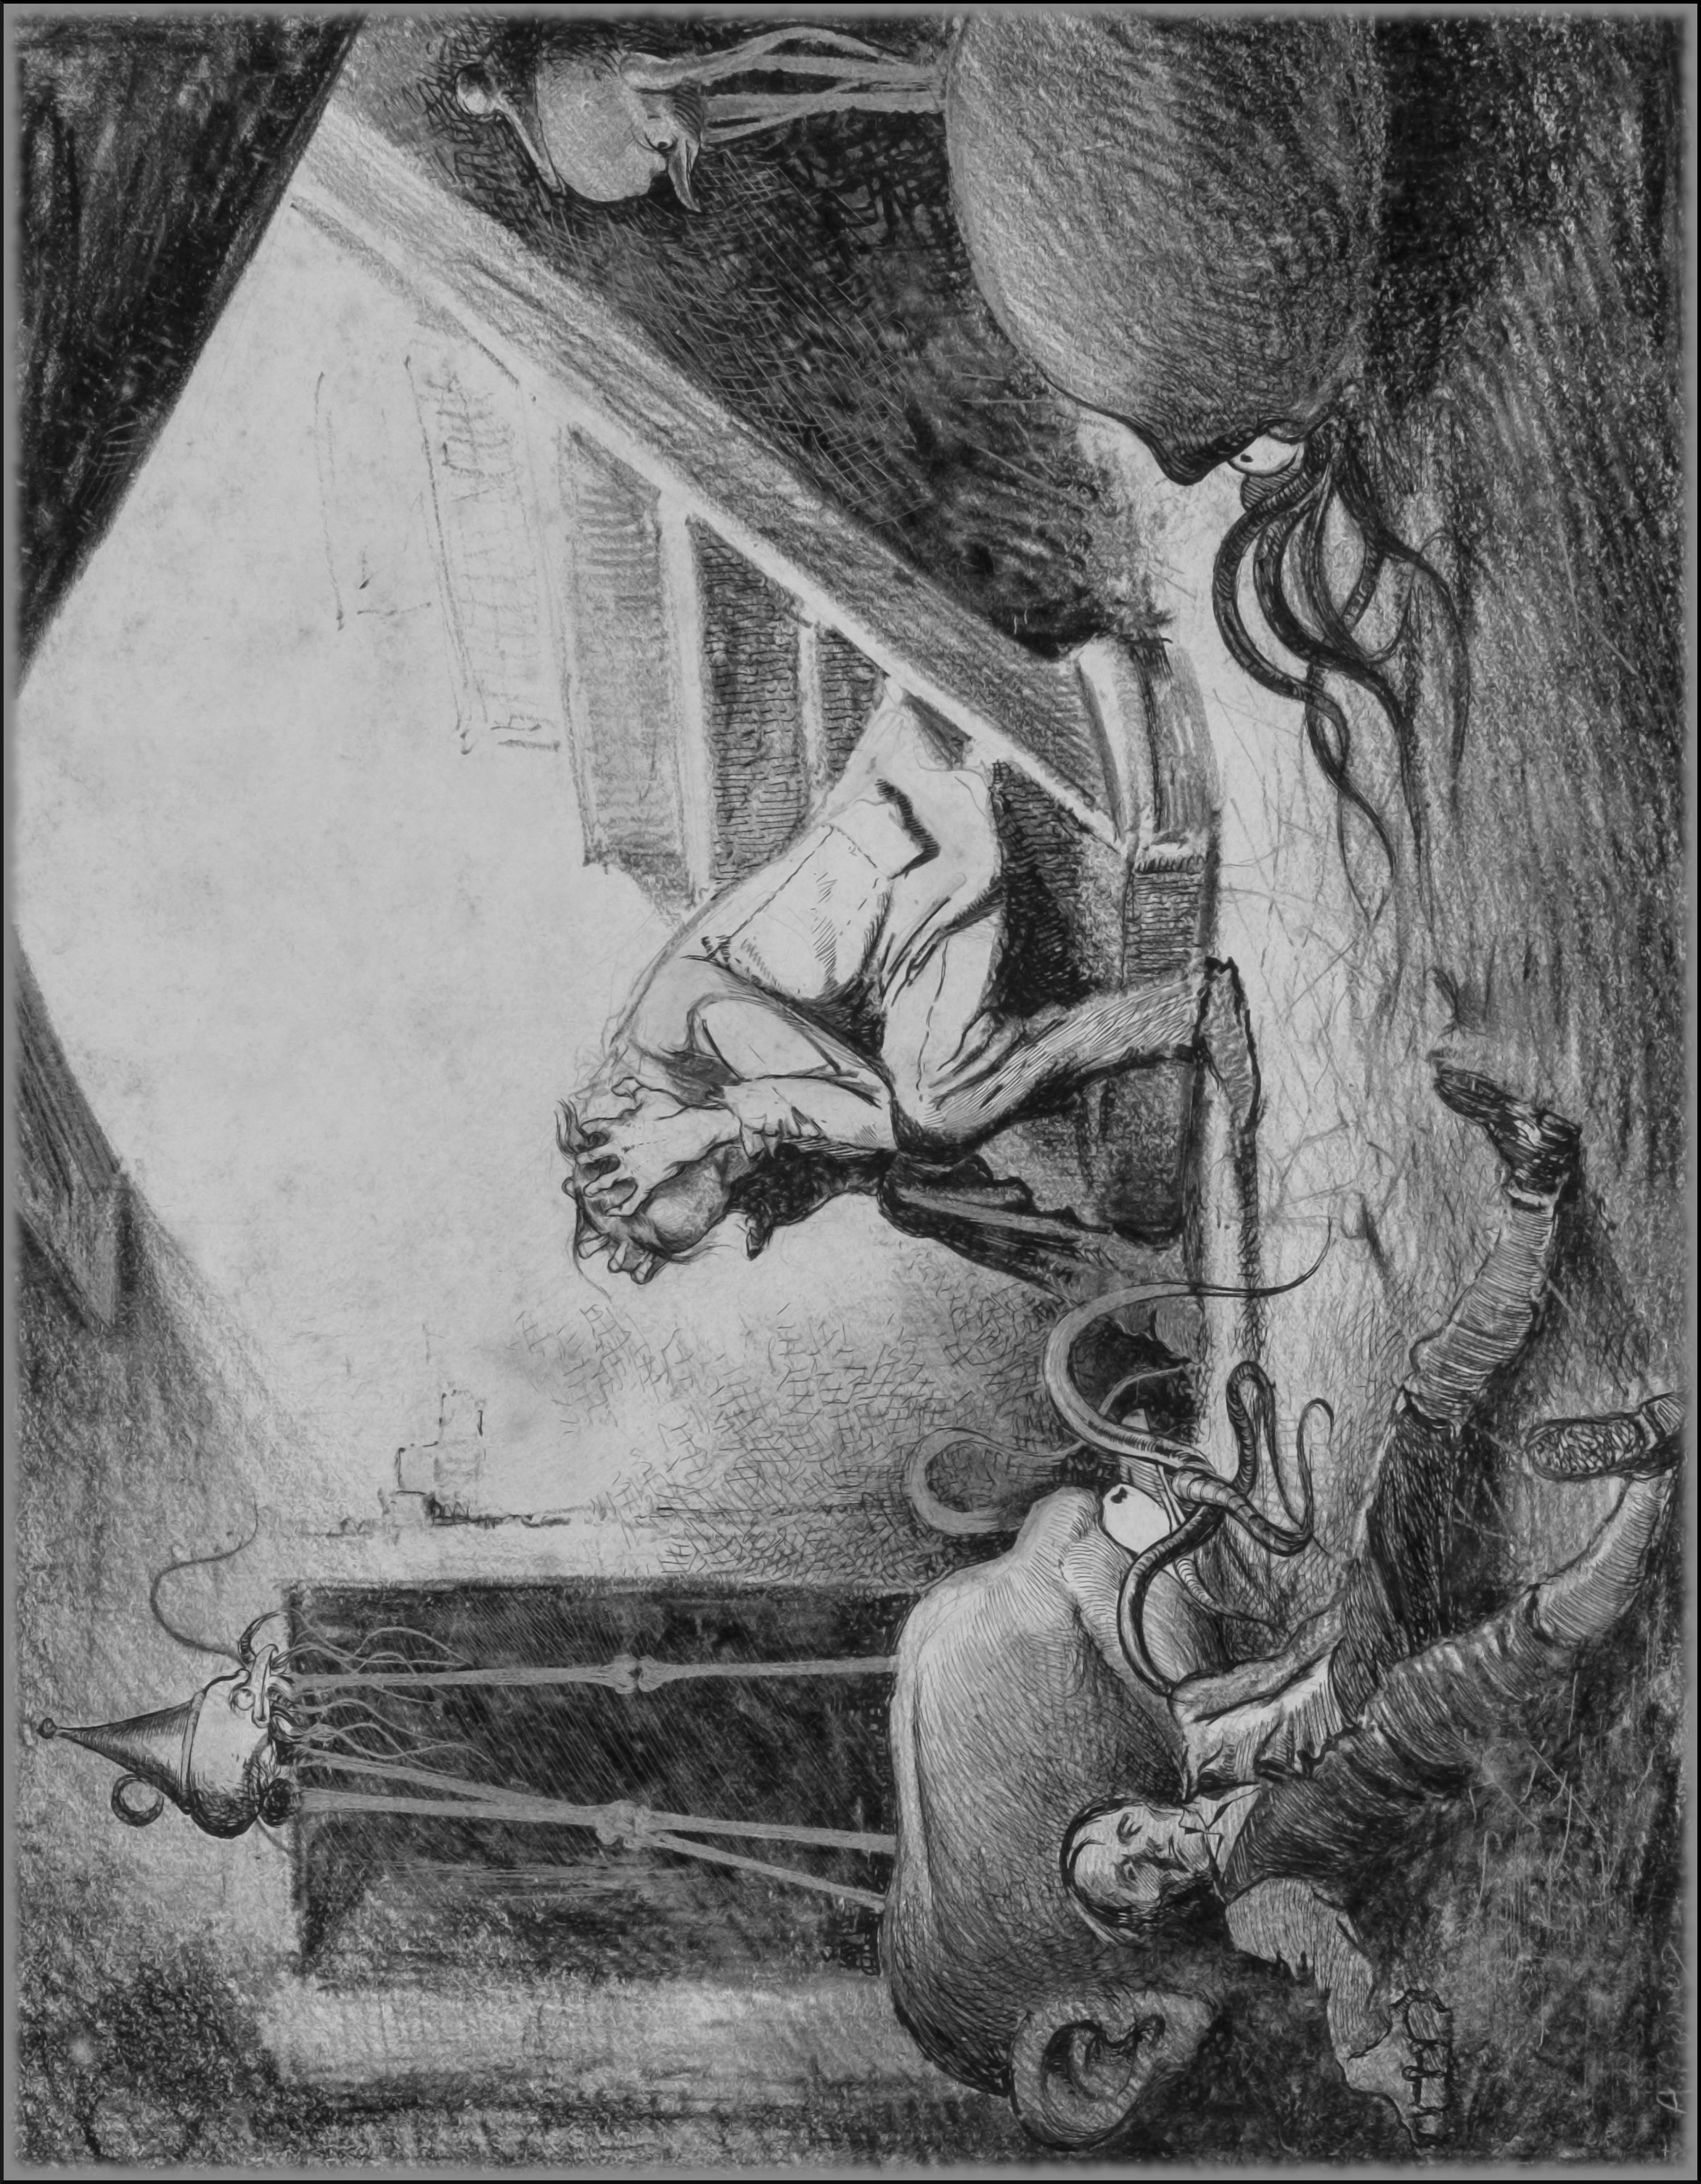
\includegraphics[width=1.15\columnwidth]{10imagination}};
			\node[rotate=90, text width=\textheight, align=center] (caption) at ($(current page.east)+(-1cm,0cm)$) {\textsc{My imagination was full of those striding metallic monsters}};

		\end{tikzpicture}
		\addxcontentsline{lof}{figure}{My imagination was full of those striding metallic monsters}
		\thispagestyle{empty}
		\clearpage
	\end{letter}

	\begin{a4}
		\clearpage
		\begin{tikzpicture}[remember picture, overlay]
			\node (img) at ($(current page.center)+(-0.5cm,0cm)$) {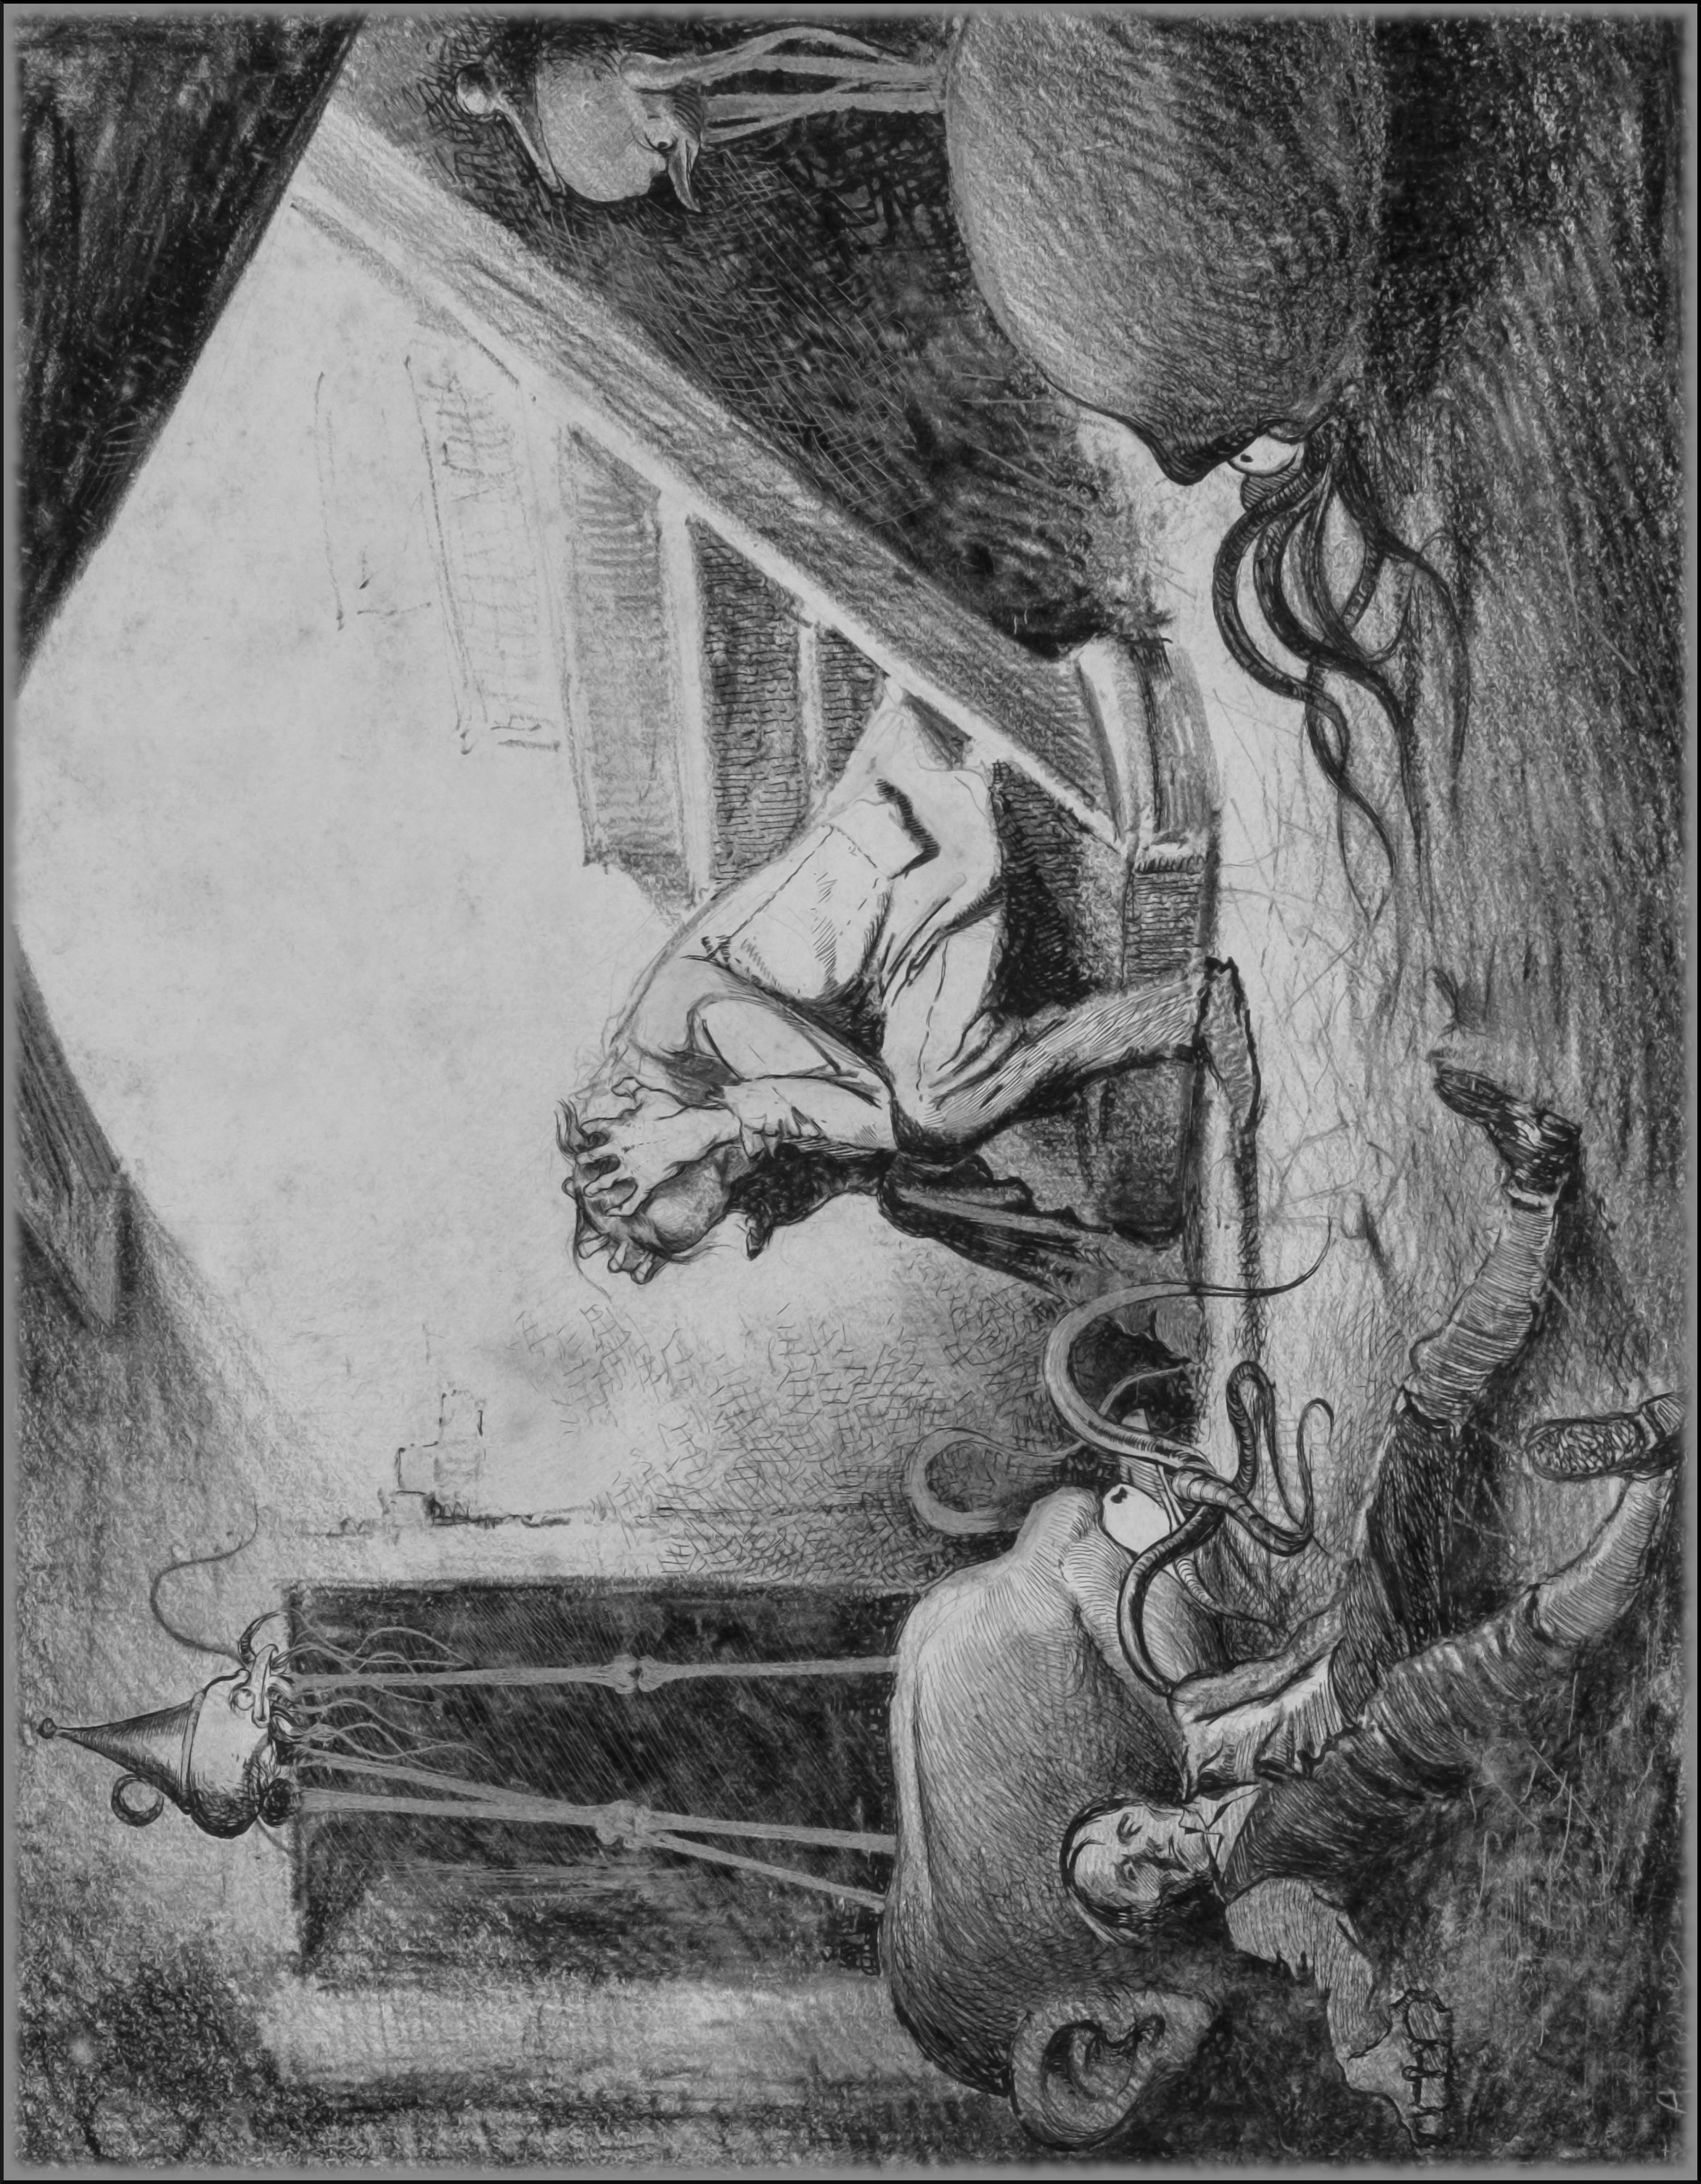
\includegraphics[width=1.15\columnwidth]{10imagination}};
			\node[rotate=90, text width=\textheight, align=center] (caption) at ($(current page.east)+(-1cm,0cm)$) {\textsc{My imagination was full of those striding metallic monsters}};

		\end{tikzpicture}
		\addxcontentsline{lof}{figure}{My imagination was full of those striding metallic monsters}
		\thispagestyle{empty}
		\clearpage
	\end{a4}
\end{pictures}



%\begin{figure}[b!]
%\centering
%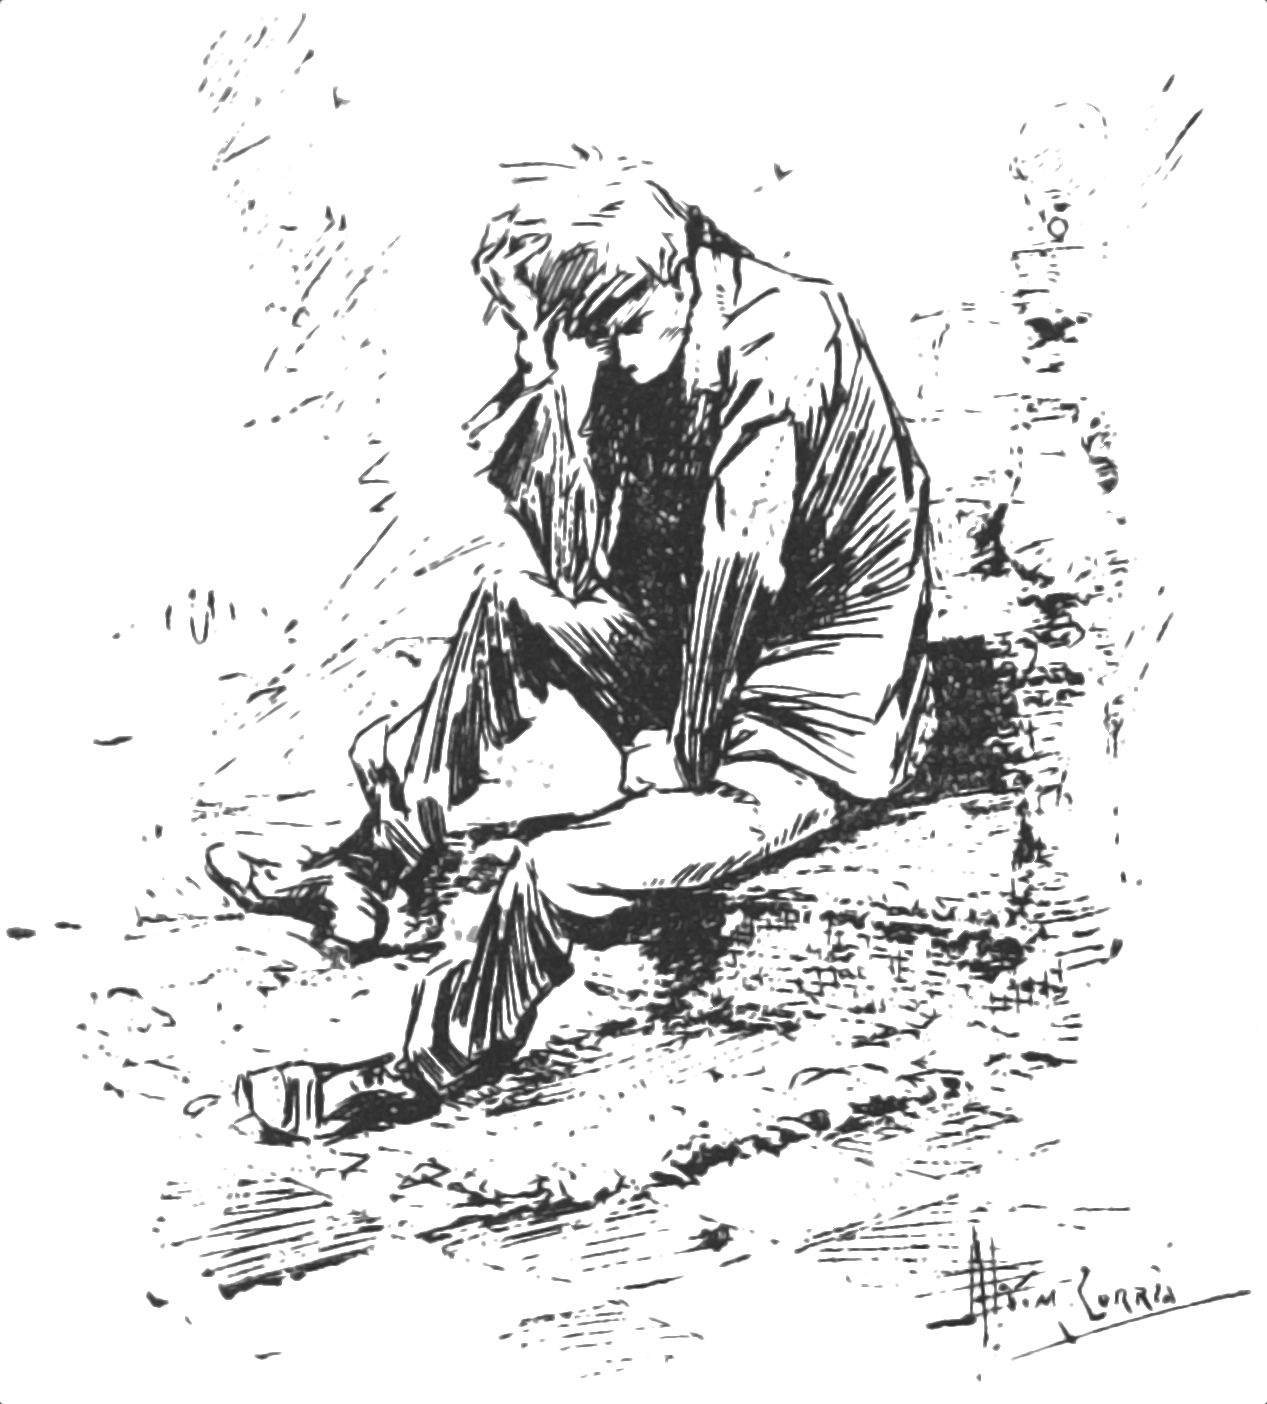
\includegraphics[width=0.7\textwidth]{10tailpiece}\captionlistentry{Tailpiece to Chapter \thechapter}
%\end{figure}